\documentclass{assignment}
\usepackage{amsmath}
\begin{document}

\assignmentTitle{Anumanchi Agastya Sai Ram Likhit}{20048}{assets/logo.png}{Computer Vision}{Assignment 1}

\section*{Question 1}
The following code explain the process of applying the filter on an image without using inbuilt libraries.
\begin{lstlisting}[language=Python]
import numpy as np
import matplotlib.pyplot as plt

def apply_filter(original_image, filter):
    image_height, image_width = original_image.shape
    filter_height, filter_width = filter.shape
    filtered_image = np.zeros_like(original_image)
 
    for i in range(1, image_height - 1):
        for j in range(1, image_width - 1):
            region = original_image[i-1:i+2, j-1:j+2]
            filtered_value = np.sum(region * filter)
            filtered_image[i, j] = filtered_value

    return filtered_image
\end{lstlisting}
  The function takes note of the dimensions  of the original image and the filter and next it creates an empty image of same shape as the original image to store the filtered image pixels,now the function iterates through the original image, skipping the border pixels, as the filter is assumed to be of size 3x3.For each pixel, a 3x3 region around it is extracted and the extracted region is multiplied by the filter matrix, and the result is summed to obtain the filtered value for the current pixel.The filtered value is assigned to the corresponding pixel in the filtered image and this way we get the Filtered image.
\\
Now below we will see how the image and the pixel values change according to the applied filters provided to us and discuss what the filters are doing.
\\
\subsection{Filter - 1}
\\
\vspace{1.4 cm}
\[\begin{bmatrix} 0 & 0 & 0 \\ 0 & 1 & 0 \\ 0 & 0 & 0 \end{bmatrix}\]
\\
\vspace{2 cm}
\begin{figure}[h]
  \begin{minipage}{0.5\textwidth}
    \centering
    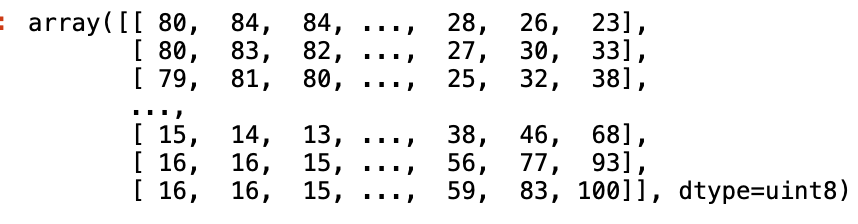
\includegraphics[width=0.8\linewidth]{image.png}
    \caption{Original Image.}
    \label{fig:original_image}
  \end{minipage}%
  \begin{minipage}{0.5\textwidth}
    \centering
    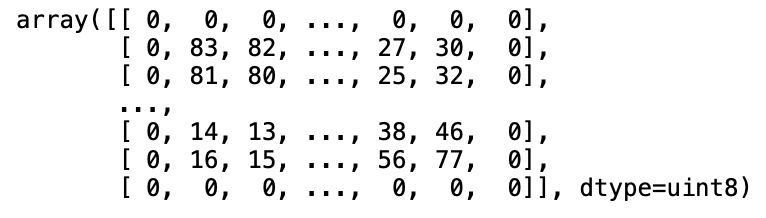
\includegraphics[width=0.8\linewidth]{f1.png}
    \caption{Filtered Image}
    \label{fig:filtered_image}
  \end{minipage}
\end{figure}
\\
This filter retains the original image, effectively doing nothing. The central value of 1 ensures that each pixel in the output will have the same value as the corresponding pixel in the input.
\begin{figure}[h]
    \centering
    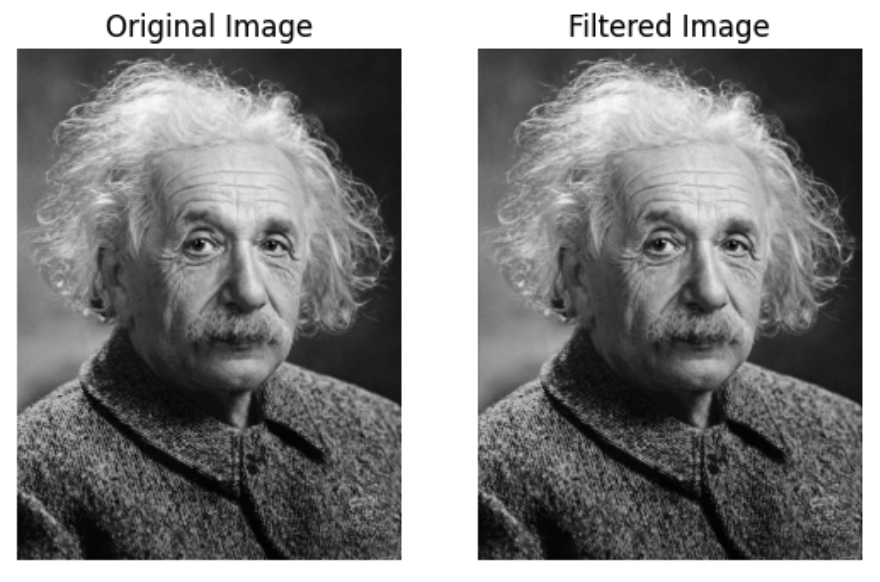
\includegraphics[width=0.4\linewidth]{magic.png}
    \caption{Comparison of original image with image after applying filter 1}
    \label{fig:enter-label}
\end{figure}
\\
If we see the image we  find no change in the image visually to the naked eye because the image size is very big and having so many pixels,the shape of the image is \((2666, 2000)\).
%%%%%%%%%%%%%%%%%%%%%%

\subsection{Filter - 2}
\[
\begin{bmatrix} 0 & 0 & 0 \\ 0 & 0 & 1 \\ 0 & 0 & 0 \end{bmatrix}
\]
\\
\begin{figure}[h]
  \begin{minipage}{0.5\textwidth}
    \centering
    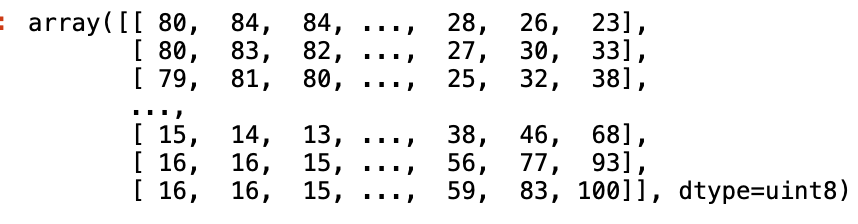
\includegraphics[width=0.8\linewidth]{image.png}
    \caption{Original Image}
    \label{fig:original_image}
  \end{minipage}%
  \begin{minipage}{0.5\textwidth}
    \centering
    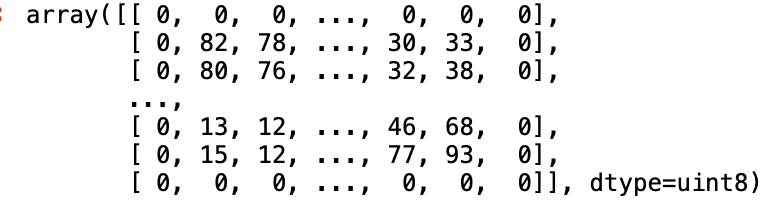
\includegraphics[width=0.8\linewidth]{f2.png}
    \caption{Filtered Image}
    \label{fig:filtered_image}
  \end{minipage}
\end{figure}
\\
This filter shifts the pixel values one position to the left, creating a motion effect towards the left.
\begin{figure}[h]
    \centering
    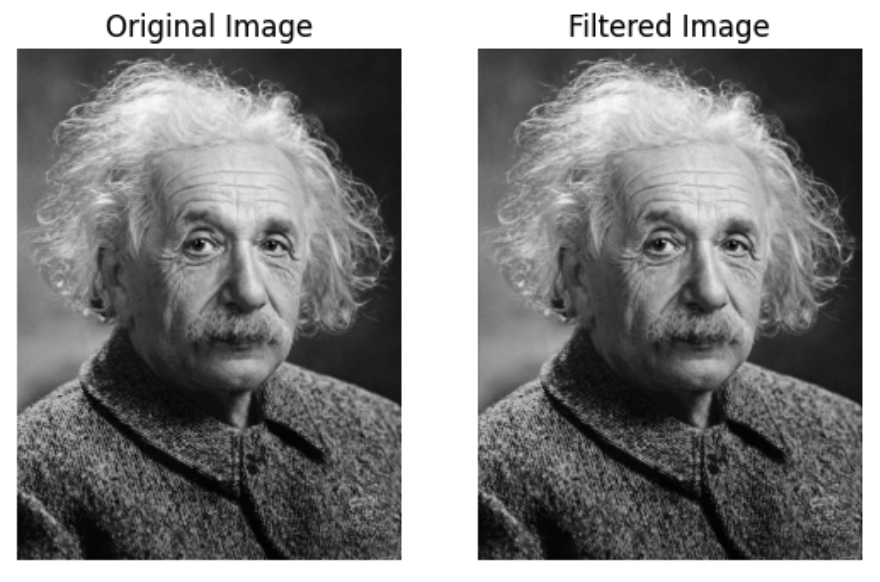
\includegraphics[width=0.4\linewidth]{magic.png}
    \caption{Comparison of original image with image after applying filter 2}
    \label{fig:enter-label}
\end{figure}
\\
If we see the image we  find no change in the image visually to the naked eye because the image size is very big and having so many pixels.

\subsection{Filter - 3}

\[
\begin{bmatrix} 0 & 0 & 0 \\ 1 & 0 & 0 \\ 0 & 0 & 0 \end{bmatrix}
\]
\\
\begin{figure}[h]
  \begin{minipage}{0.5\textwidth}
    \centering
    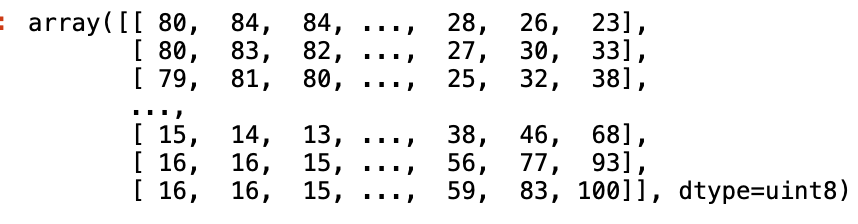
\includegraphics[width=0.8\linewidth]{image.png}
    \caption{Original Image}
    \label{fig:original_image}
  \end{minipage}%
  \begin{minipage}{0.5\textwidth}
    \centering
    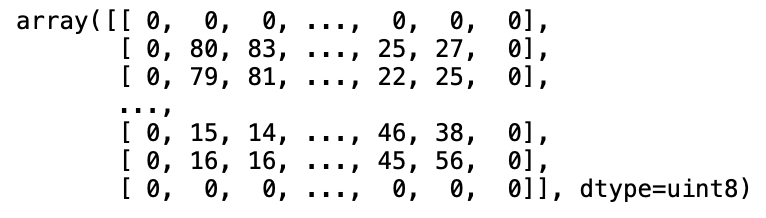
\includegraphics[width=0.8\linewidth]{f3.png}
    \caption{Filtered Image}
    \label{fig:filtered_image}
  \end{minipage}
\end{figure}
\\

This filter shifts the pixel values one position to the right, creating a motion effect towards the right.
\begin{figure}[h]
    \centering
    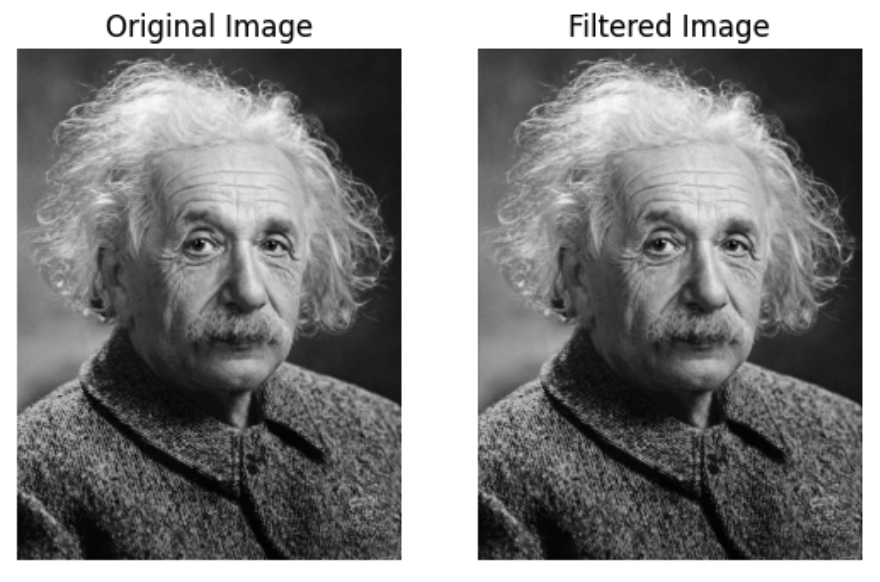
\includegraphics[width=0.4\linewidth]{magic.png}
    \caption{Comparison of original image with image after applying filter 3}
    \label{fig:enter-label}
\end{figure}
\\
If we see the image we  find no change in the image visually to the naked eye because the image size is very big and having so many pixels.
\newpage
\subsection{Filter - 4}
\[
\begin{bmatrix} 0 & 0 & 1 \\ 0 & 0 & 0 \\ 0 & 0 & 0 \end{bmatrix}
\]
\\
\begin{figure}[h]
  \begin{minipage}{0.5\textwidth}
    \centering
    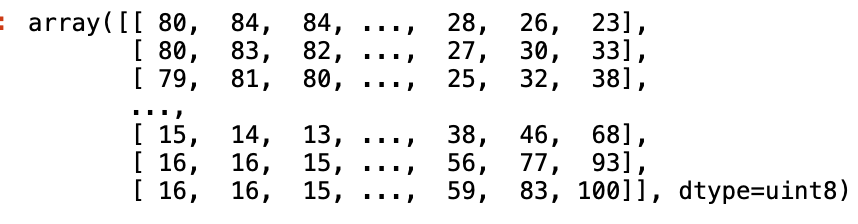
\includegraphics[width=0.8\linewidth]{image.png}
    \caption{Original Image}
    \label{fig:original_image}
  \end{minipage}%
  \begin{minipage}{0.5\textwidth}
    \centering
    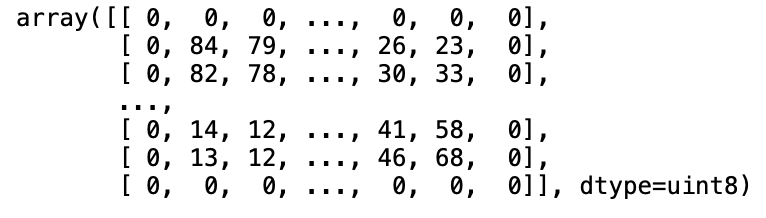
\includegraphics[width=0.8\linewidth]{f4.png}
    \caption{Filtered Image}
    \label{fig:filtered_image}
  \end{minipage}
\end{figure}
\\
This filter shifts the pixel values one position upward to the right, creating a unique spatial transformation.
\begin{figure}[h]
    \centering
    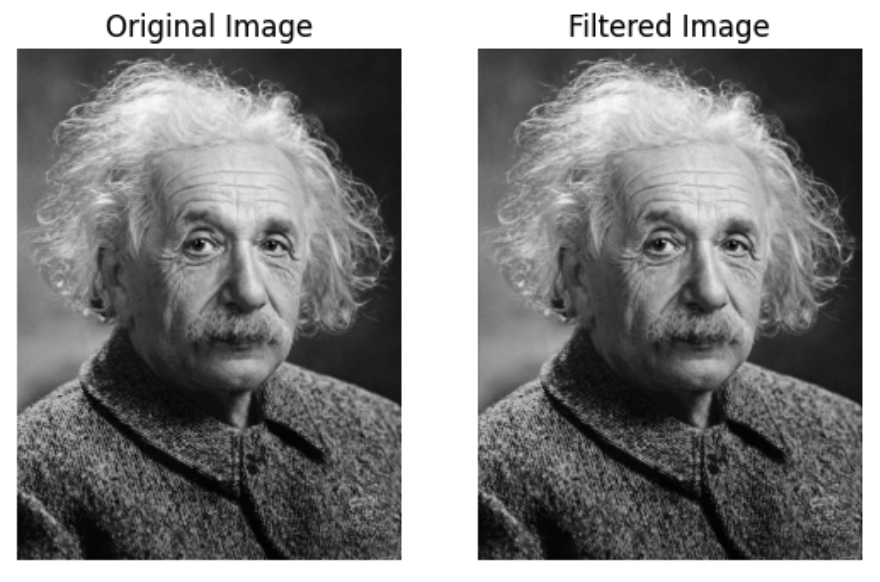
\includegraphics[width=0.5\linewidth]{magic.png}
    \caption{Comparison of original image with image after applying filter 4}
    \label{fig:enter-label}
\end{figure}
\\
If we see the image we  find no change in the image visually to the naked eye because the image size is very big and having so many pixels.
\subsection{Filter - 5}
\[
\begin{bmatrix} 0 & 0 & 0 \\ 0 & 0 & 0 \\ 1 & 0 & 0 \end{bmatrix}
\]
\\
\begin{figure}[h]
  \begin{minipage}{0.5\textwidth}
    \centering
    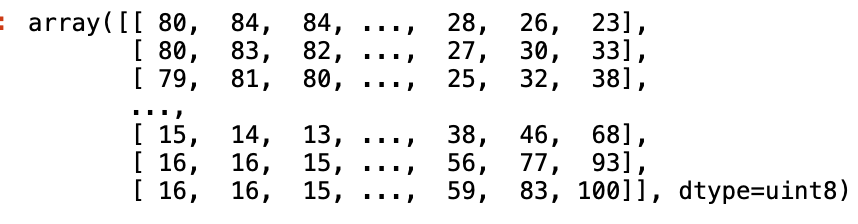
\includegraphics[width=0.8\linewidth]{image.png}
    \caption{Original Image}
    \label{fig:original_image}
  \end{minipage}%
  \begin{minipage}{0.5\textwidth}
    \centering
    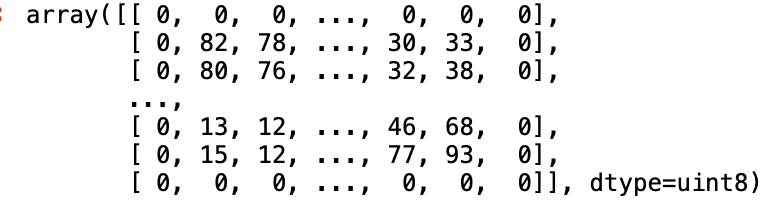
\includegraphics[width=0.8\linewidth]{f2.png}
    \caption{Filtered Image}
    \label{fig:filtered_image}
  \end{minipage}
\end{figure}
\\
This filter shifts the pixel values one position downward to the right, creating a diagonal shifting effect.
\\
\begin{figure}[h]
    \centering
    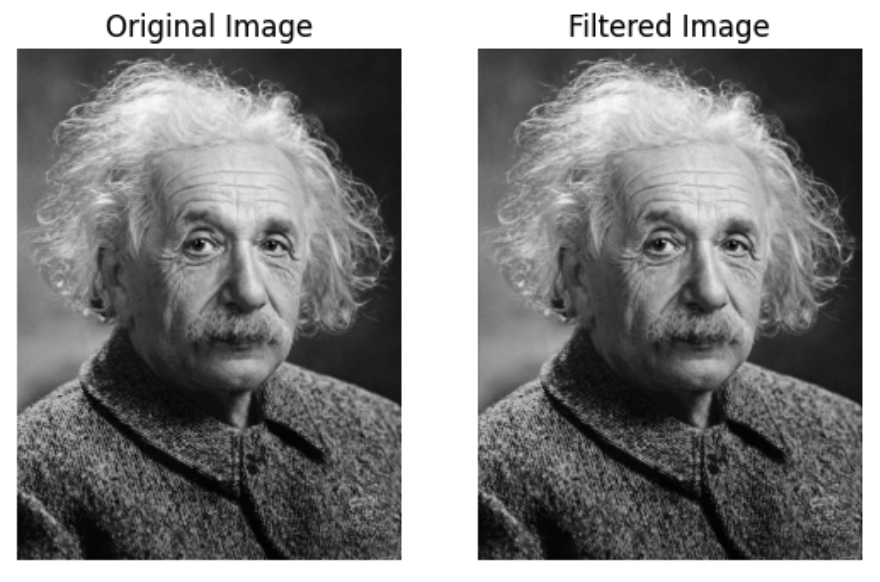
\includegraphics[width=0.5\linewidth]{magic.png}
    \caption{Comparison of original image with image after applying filter 5}
    \label{fig:enter-label}
\end{figure}
\\
If we see the image we  find no change in the image visually to the naked eye because the image size is very big and having so many pixels.
\section*{Question 2}
\subsection{Filter 1}
\[
\begin{bmatrix} 1 & 0 & -1 \\ 2 & 0 & -2 \\ 1 & 0 & -1 \end{bmatrix}
\]
\\
\begin{figure}[h]
    \centering
    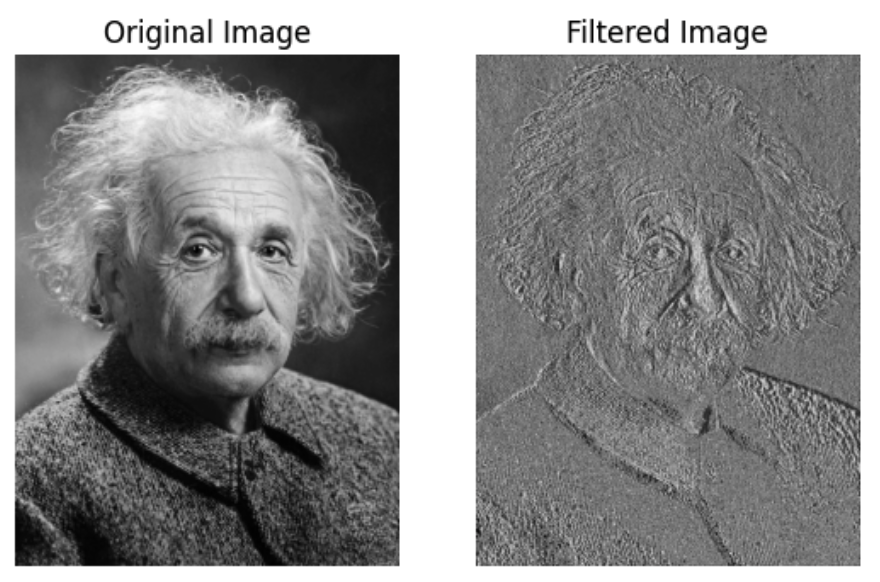
\includegraphics[width=0.5\linewidth]{2_1.png}
    \caption{Comparison of original image with image after applying Vertical Sobel filter}
    \label{fig:enter-label}
\end{figure}
\\
When this filter is applied to an image,The positive values on the left side of the filter are used to detect vertical edges where the intensity increases from left to right,while the negative values on the right side of the filter are used to detect vertical edges where the intensity decreases from left to right,this filter is called Sobel filter and its more used in detecting edges and more particularly vertical edges within an image.

\subsection{Filter 2}
\[
\begin{bmatrix} 1 & 2 & 1 \\ 0 & 0 & 0 \\ -1 & -2 & -1 \end{bmatrix}
\]
\\
\begin{figure}[h]
    \centering
    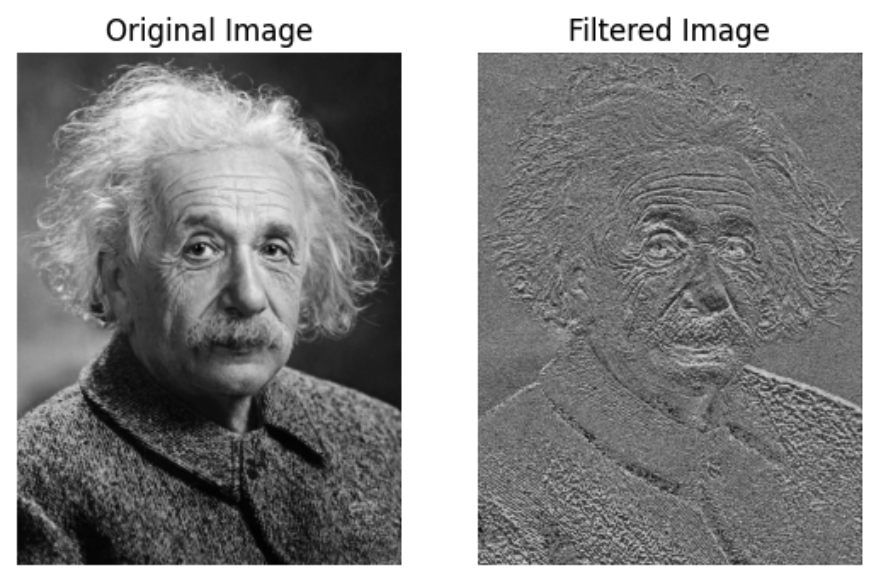
\includegraphics[width=0.5\linewidth]{2_2.png}
    \caption{Comparison of original image with image after applying filter Horizontal Sobel filter}
    \label{fig:enter-label}
\end{figure}
\\
When this filter is applied to an image,The positive values on the top side of the filter are used to detect horizontal edges where the intensity increases from top to bottom,while the negative values on the bottom side of the filter are used to detect horizontal edges where the intensity decreases from top to bottom,this filter is also called Sobel filter and its more used in detecting edges and more particularly horizontal edges within an image.
\section*{Question 3}
\subsection{Filter 1}
\[
\frac{1}{9}\begin{bmatrix} 1 & 1 & 1 \\ 1 & 1 & 1 \\ 1 & 1 & 1 \end{bmatrix}
\]
\\
\begin{figure}[h]
  \begin{minipage}{0.5\textwidth}
    \centering
    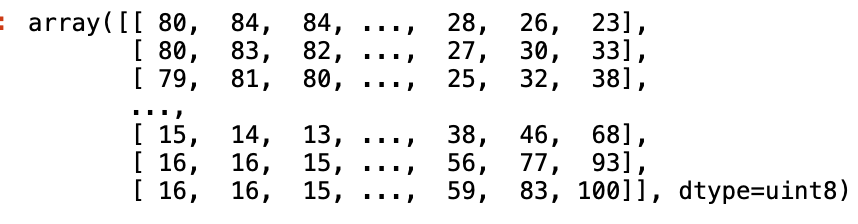
\includegraphics[width=0.8\linewidth]{image.png}
    \caption{Original Image}
    \label{fig:original_image}
  \end{minipage}%
  \begin{minipage}{0.5\textwidth}
    \centering
    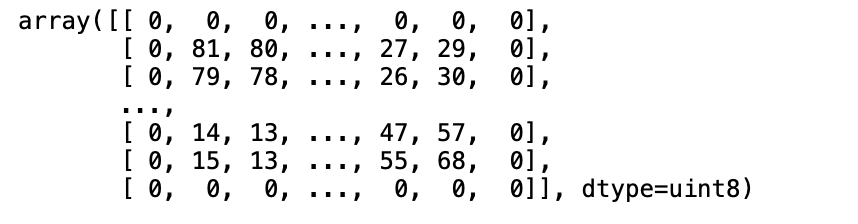
\includegraphics[width=0.8\linewidth]{f3_1.png}
    \caption{Filtered Image}
    \label{fig:filtered_image}
  \end{minipage}
\end{figure}
\\
it takes the average of the pixel values in a \(3 \times 3\) neighborhood around each pixel in the original image.Specifically, it adds up the values of a pixel and its eight immediate neighbors, then divides the sum by 9,that is it simply replaces the image pixel with the average of the surrounding pixel values.

The effect of this filter is to smooth the image, reducing sharp edges and noise.
\\
\begin{figure}[h]
    \centering
    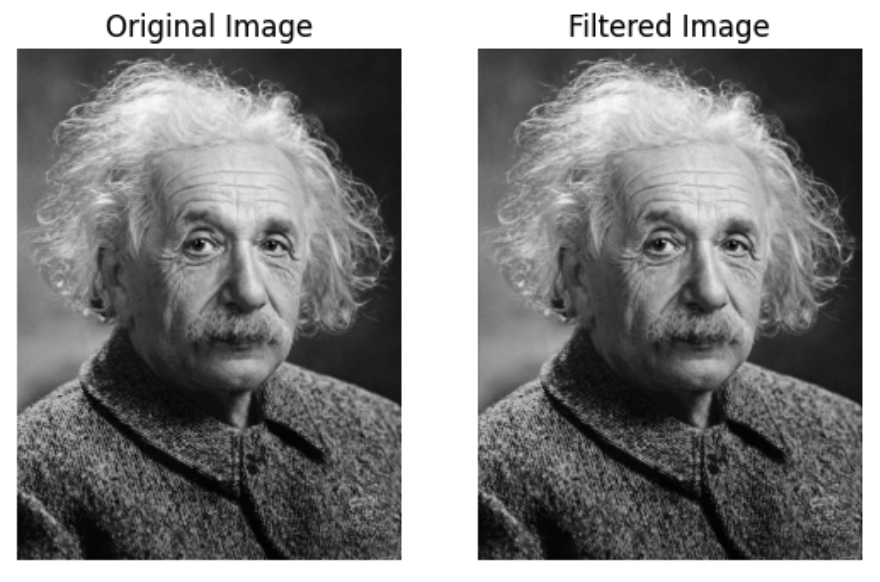
\includegraphics[width=0.4\linewidth]{magic.png}
    \caption{Comparison of original image with image after applying filter}
    \label{fig:enter-label}
\end{figure}
\\
\subsection{Filter 2}
\[
\frac{1}{15}\begin{bmatrix} 1 & 2 & 1 \\ 2 & 3 & 2 \\ 1 & 2 & 1 \end{bmatrix}
\]
\\
\begin{figure}[h]
  \begin{minipage}{0.5\textwidth}
    \centering
    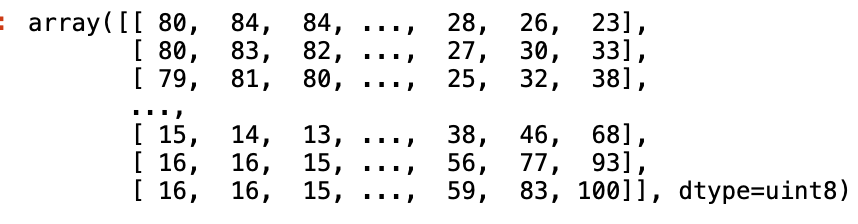
\includegraphics[width=0.8\linewidth]{image.png}
    \caption{Original Image}
    \label{fig:original_image}
  \end{minipage}%
  \begin{minipage}{0.5\textwidth}
    \centering
    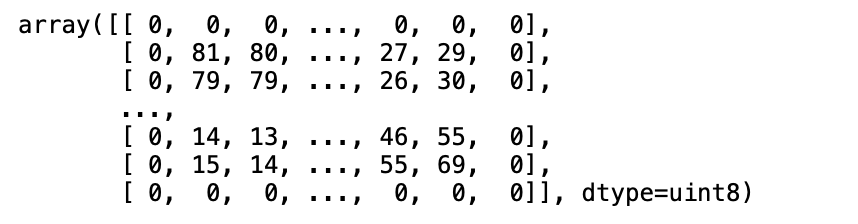
\includegraphics[width=0.8\linewidth]{f3_2.png}
    \caption{Filtered Image}
    \label{fig:filtered_image}
  \end{minipage}
\end{figure}
\\
This is an Gaussian filter this also does the same job as the above filter,it does averaging but giving different weights to the surrounding pixel values.
\\
\\
\begin{figure}[h]
    \centering
    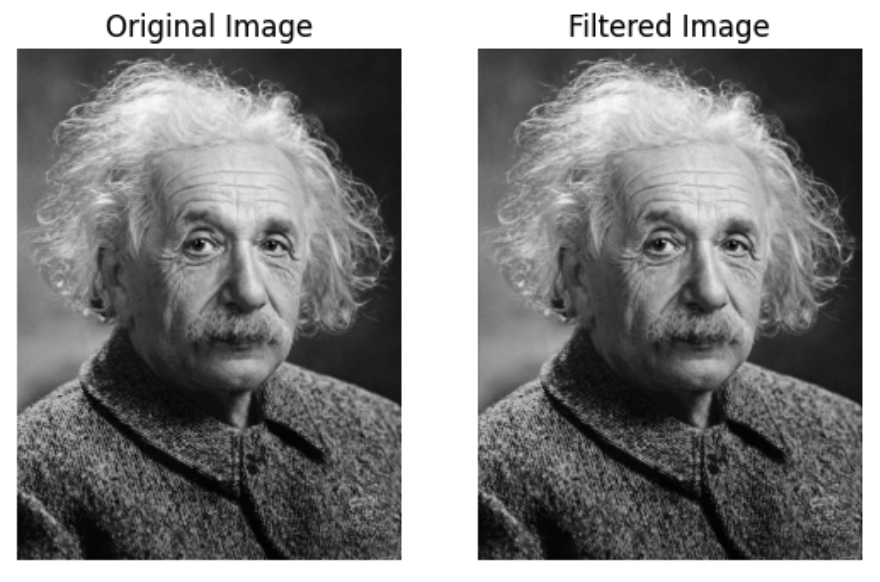
\includegraphics[width=0.4\linewidth]{magic.png}
    \caption{Comparison of original image with image after applying filter}
    \label{fig:enter-label}
\end{figure}
\\
But here due to the large number of pixels of the image we cant see the noticable change.
\end{document}
